\documentclass[10pt]{article}
\usepackage[english]{babel}
\usepackage[utf8]{inputenc}
\usepackage{amsmath}
\usepackage{listings}
\usepackage{tikz}
\usepackage{tkz-euclide}

\title{\vspace{-5.0cm}LaTeX tkz-euclide EXAMPLES}
\author{\vspace{-0.1cm}Jeff DeCola}
\date{\vspace{-1.0cm}}

\setlength{\parindent}{0em} %Paragraph Indent
\setlength{\parskip}{1em} %Paragraph Spacing

\begin{document}
\maketitle

\textbf{This will draw a coordinate plane,}

\begin{lstlisting}
\resizebox{8cm}{8cm}{%
    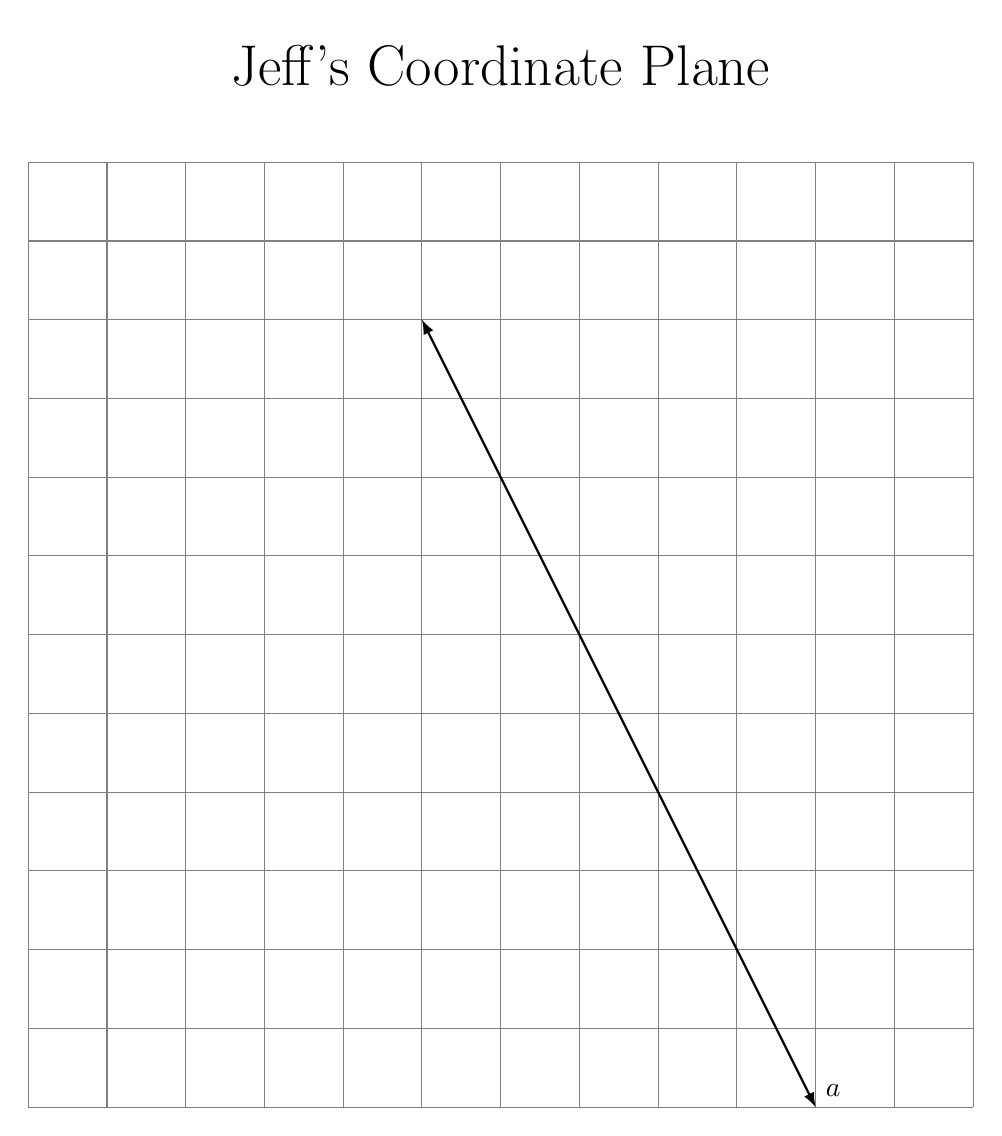
\begin{tikzpicture}
        \tkzInit[xmax=6,ymax=6,xmin=-6,ymin=-6]
        \tkzGrid
        \tkzAxeXY
        \draw[ thick,latex-latex] (-1,4) -- (4,-6) node[anchor=south west] {$a$}; % two points for drawing 2x+y=2
        \huge\tkzText[above](0,6.75){Jeff's Coordinate Plane}
    \end{tikzpicture}
}
\end{lstlisting}

\begin{center}
\resizebox{8cm}{8cm}{%
    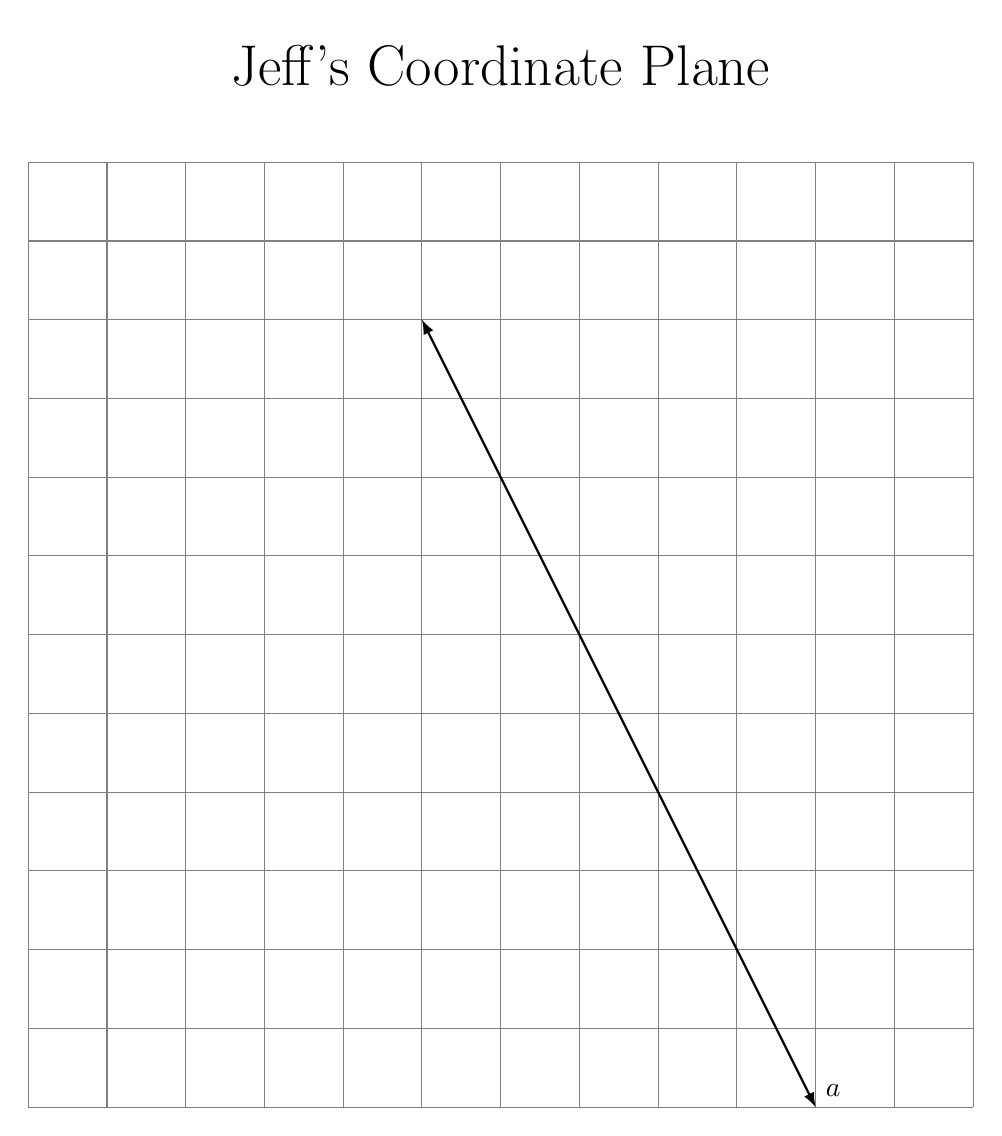
\begin{tikzpicture}
        \tkzInit[xmax=6,ymax=6,xmin=-6,ymin=-6]
        \tkzGrid
        \tkzAxeXY
        \draw[ thick,latex-latex] (-1,4) -- (4,-6) node[anchor=south west] {$a$}; % two points for drawing 2x+y=2
        \huge\tkzText[above](0,6.75){Jeff's Coordinate Plane}
    \end{tikzpicture}
}
\end{center}

\end{document}







